\begin{figure}[!htbp]
\centering
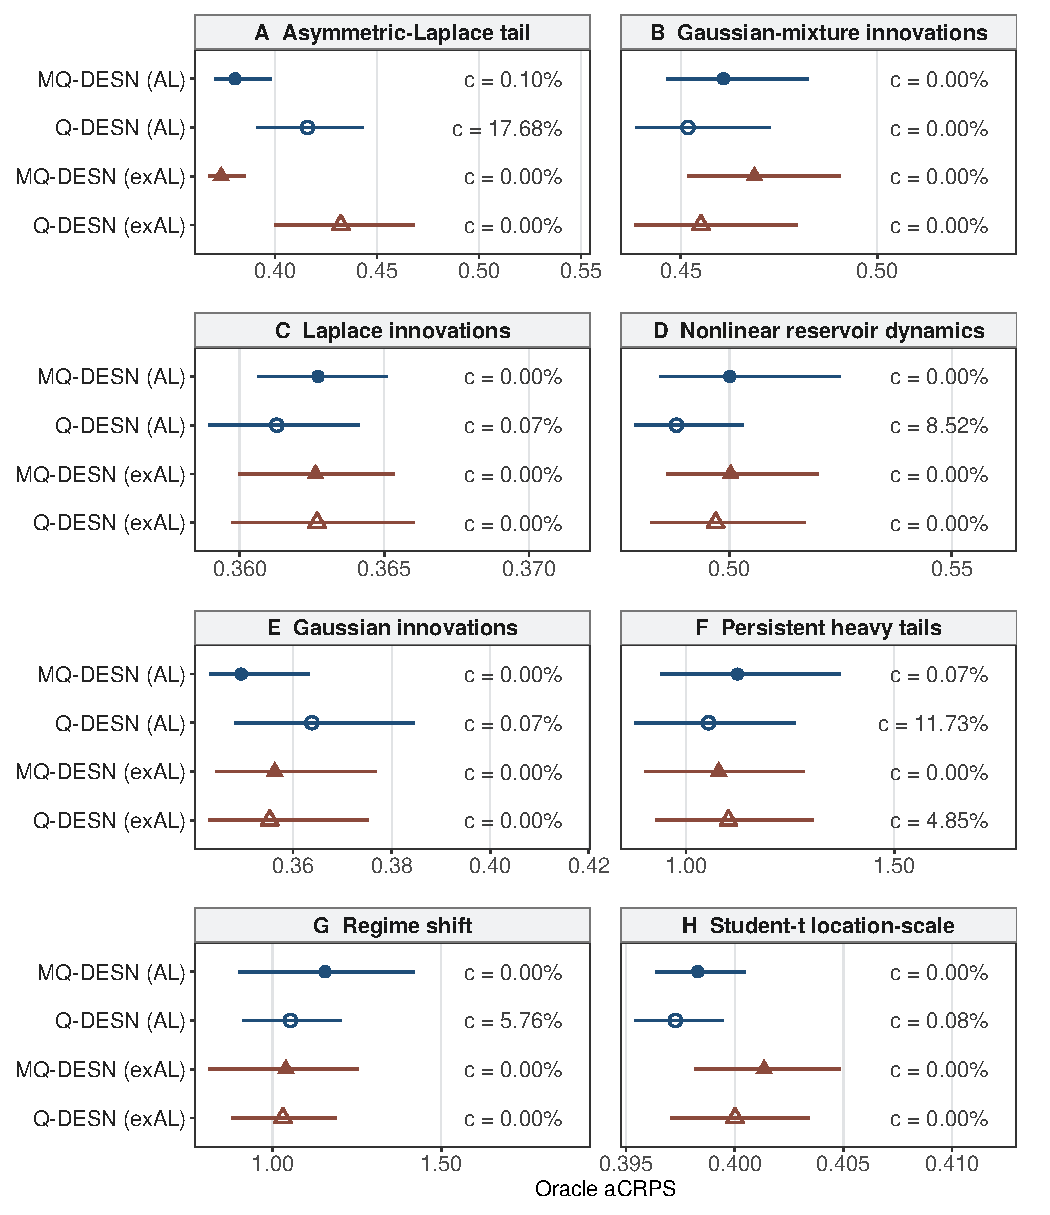
\includegraphics[width=0.94\textwidth]{figures/joint_qdesn_simulation/joint_qdesn_pure_desn_v2_mq_forecast_dgp_acrps.pdf}
\caption{Oracle finite-grid \(\aCRPS\) in the multiquantile study. Points are posterior means and segments are equal-tailed 95\% intervals for the score averaged over the common forecast pairs, conditional on each model's averaged recursive future features. Lower scores are better. Annotations \(c\) give raw adjacent-level crossing percentages for posterior-mean forecast grids. Q--DESN fits levels independently; MQ--DESN estimates their coefficients jointly. The scored grids use the monotone transformation specified in the supplement.}
\label{fig:joint-qdesn-pure-desn-v2-forecast-acrps}
\end{figure}
